%+----------------------------------------------------------------------------+
%| SLIDES: PostDoc interview presentation
%| Duration: 20 minutes
%| Contents: 7 slides
%|					 (extimated duration 3 minutes per slide )
%| Author: Antonio miti
%| Place: Brescia, January 2023
%+----------------------------------------------------------------------------+



%- HandOut Flag -----------------------------------------------------------------------------------------
\newif\ifHandout
	\Handouttrue  %uncomment for the printable version


%- D0cum3nt ----------------------------------------------------------------------------------------------
\ifHandout
	\documentclass[handout,10pt]{beamer}   
	\setbeameroption{show notes} %print notes   
\else
	\documentclass[10pt]{beamer}
\fi

	
%- Packages ----------------------------------------------------------------------------------------------
\usepackage{./custom-style}
\usepackage{./math}
\usepackage{textpos,eso-pic}
\usepackage{fontawesome}


%--Beamer Style-----------------------------------------------------------------------------------------------
\usetheme{toninus}

%- Macros -------------------------------------------------------------------------------------------
\providecommand{\vHam}{\mathscr{v}}


\renewcommand{\checkpoint}[0]{
	\setcounter{tocdepth}{2}
	\addtocounter{framenumber}{-1}
 	\begin{frame}[t]{Outline}
			\tableofcontents[currentsection,currentsubsection]
	\end{frame}
}


%- TEMP -----------------------------------------------------------------------------
\newtcolorbox[auto counter,number within=section]{probox}[2][]{%
	fonttitle= \footnotesize \bfseries,
	title=#2,
	fontupper=\footnotesize,%\sffamily,
	colback=white,
	colbacktitle=white,
	coltitle=orange!70!black,
	colframe=orange!70!black,
	%boxrule=1pt,
	titlerule=0pt,
	toptitle=-0.2em,bottomtitle=-0.2em, %title spacing	
	colback=white,
	leftupper=-3mm,rightupper=0mm,top=0mm,bottom=0mm, 
	#1,
}

\renewcommand{\action}{\curvearrowright}


%- T1tle P4g3 -------------------------------------------------------------------------------------------
\title{\LARGE Research overview \vspace{-.5em}} 
%\subtitle{}
\author[AMM]{\large \href{https://dmf.unicatt.it/miti/}{Antonio Michele Miti}}
\institute[UCSC]{
	\vspace{1em}
	\\
	Dipartimento di Matematica e Fisica,\\
	Universit\'a Cattolica del Sacro Cuore, 
	Brescia, Italy 
	\\
	\href{https://www.mpim-bonn.mpg.de/}{
\includegraphics[width=5cm]{./Logos/Ucsc_logo}}
	\vspace{1em}
}
\date[Mpim_22] % (optional, should be abbreviation of conference name)
{	
	{\vskip 1ex}
	Unimib Interview, February 8, 2023
}


%---------------------------------------------------------------------------------------------------------------------------------------------------
%- D0cum3nt ----------------------------------------------------------------------------------------------------------------------------------
\begin{document}
%------------------------------------------------------------------------------------------------

%-------------------------------------------------------------------------------------------------------------------------------------------------
\maketitle
%-------------------------------------------------------------------------------------------------------------------------------------------------


%-------------------------------------------------------------------------------------------------------------------------------------------------
\begin{frame}[fragile]{Project title}
\tikzstyle{every picture}+=[remember picture]
	\begin{columns}
    	\begin{column}{.45\textwidth}
    		\onslide<4->{
			\tikz[baseline]{
		            \node[draw=orange!40,anchor=base,text width=5cm] (s1)
		            {Group of transformations preserving the prescribed geometric structures.};
			}
		}
	\end{column}
    	\begin{column}{.45\textwidth}
    		\onslide<5->{
			 \tikz[baseline]{
		            \node[draw=blue!40,anchor=base, text width=5cm] (s2)
		            {Procedure providing another manifold of reduced dimension encoding the relevant geometrical information.};
			}
		}
	\end{column}
	\end{columns}

	\vfill

	\begin{center}
		\large
		 \tikz[baseline]{
		            \node[fill=orange!20,anchor=base] (t1)
		            {Multisymplectic manifolds};
			}
		 , 
		 \tikz[baseline]{
		            \node[fill=blue!20,anchor=base] (t2)
		            {homotopy comomentum maps};
		        } 
		, 
		\\
		 \tikz[baseline]{
	            \node[fill=green!20,anchor=base] (t3)
	            {$L_\infty$-algebras};
		}
		, and
		 \tikz[baseline]{
	            \node[fill=red!20,anchor=base] (t4)
	            {applications};
		}		
	\end{center}

	\vfill

	\begin{columns}
    	\begin{column}{.45\textwidth}
    		\onslide<3->{
	 		 \tikz[baseline]{
	            \node[draw=green!40,anchor=base,text width=5cm] (s3)
	            {A certain higher version \\(involving differential forms in degree $\geq 2$)};
	         }
		}		   	
		\end{column}
    	\begin{column}{.45\textwidth}
    		\onslide<2->{
				\tikz[baseline]{
	            \node[draw=red!40,anchor=base,text width=5cm] (s4)
	            {Geometric structure providing a prescription on how to measure the area of 2-dimensional surface elements embedded in the manifold.};
	           }	
			}
		\end{column}
	\end{columns}

	\begin{tikzpicture}[overlay]
        \path[->,draw=orange!40]<4-> (s1) edge [bend right] (t1);
        \path[->,draw=blue!40]<5-> (s2) edge [bend left] (t2);
        \path[->,draw=green!40]<3-> (s3) edge [bend left] (t3);
        \path[->,draw=red!40]<2-> (s4) edge [bend right] (t4);
	\end{tikzpicture}


\end{frame}
\note[itemize]{
	\item Provide a vague idea of the words that make up the title.
	\item
	\item Conventions:
	\\- $M$ and $G$ are connected,
	\\- actions $\theta:G \curvearrowright M$ are always smooth
	\\- $\xi,\eta\in\mathfrak{g}$,
	\\- for $\mu\in\Omega^*(M,\mathfrak{g}^*)$ and $\xi\in\mathfrak{g}$, write
			\[
				\mu_\xi := \langle\mu,\xi\rangle \;{\color{black!50}\in\Omega^*(M)}
			\]
			for the ``$\xi$th component'' of $\mu$.
}
%-------------------------------------------------------------------------------------------------------------------------------------------------


%-------------------------------------------------------------------------------------------------------------------------------------------------
\section{Research Statement}
%-------------------------------------------------------------------------------------------------------------------------------------------------
%-------------------------------------------------------------------------------------------------------------------------------------------------
\subsection{Framework}
\checkpoint
%-------------------------------------------------------------------------------------------------------------------------------------------------

%-------------------------------------------------------------------------------------------------------------------------------------------------
\begin{frame}[t, fragile]{Research Framework:  \textbf{multisymplectic geometry}} %Fragile -->workaround tikzcd
	\begin{center}
		$-$ \emph{multisymplectic means \textbf{going higher} in the degree of $\omega$} $-$
	\end{center}
	\pause
	\begin{defblock}[$n$-plectic manifold ~\emph{(Cantrijn, Ibort, De Le\'on)} \cite{Cantrun2017}]
		\includestandalone[width=0.95\textwidth]{./Pictures/Figure_multisym}	
	\end{defblock}
	%
	\vfill
	%
	%
	\pause
	\begin{block}{Examples:}
		\begin{itemize}
			\item[$\bullet$] 1-plectic $=$ symplectic
			\item[$\bullet$] Any oriented $(n+1)$-dimensional manifold is $n$-plectic w.r.t. the volume form.
			\item[$\bullet$] The multicotangent bundle $\Lambda^n T^\ast Q$ is naturally $n$-plectic.
		\end{itemize}
	\end{block}			 
%
	\pause
	\begin{block}{Historical motivation}
		Mechanics: geometrical foundations of \textit{(first-order)} field theories.
		\begin{itemize}
		 \item[•] Kijowski, W. Tulczyjew \cite{Kijowski1979}; %(1979)
		 \item[•] Cariñena, Crampin, Ibort \cite{Carinena1991b};% (1991)
		 \item[•] Gotay, Isenberg, Marsden, Montgomery \cite{Gimmsy1};%(1998)
		 \\ $\cdots$
		\end{itemize}
	\end{block}
\end{frame}
%-------------------------------------------------------------------------------------------------------------------------------------------------


%-------------------------------------------------------------------------------------------------------------------------------------------------
\begin{frame}{Observables in \textbf{multisymplectic geometry}}
	%
	\begin{defblock}[Hamiltonian $(n-1)$-forms]
		\begin{displaymath}
			\Omega^{n-1}_{ham}(M,\omega) 	:=
			\biggr\{ \sigma \in  \Omega^{n-1}(M) \; \biggr\vert \; 
				\exists \vHam_\sigma \in \mathfrak{X}(M) ~:~ 
				\tikz[baseline,remember picture]{\node[rounded corners,
                        fill=orange!5,draw=orange!30,anchor=base]            
            			(target) {$d \sigma = -\iota_{\vHam_\sigma} \omega$ };
            	}				
				~\biggr\} 
			\end{displaymath}
	\end{defblock}
	%
	\onslide<2>{
		\tikz[overlay,remember picture]
		{
			\node[rounded corners,
                 fill=orange!5,draw=orange!30,anchor=base]
            	 (base) at ($(current page.north east)-(2,1)$) [rotate=-0,text width=3.5cm,align=center] {\footnotesize{\textcolor{red}{Hamilton-DeDonder-Weyl \\equation}}};
		}	
		\begin{tikzpicture}[overlay,remember picture]
		    	\path[->] (base.south east) edge[bend left,red](target.east);
	    \end{tikzpicture}
	}
	%
	\vspace{-1em}
	\pause
	\begin{columns}[T]
		\setlength{\belowdisplayskip}{5pt}
		\begin{column}{.50\linewidth}
			%
			\centering \it
			$-$ symplectic case $-$
			\onslide<3->{
			\begin{thmblock}[Observables Poisson algebra]
				$C^\infty(M,\omega)$ endowed with
				\vspace{-.5em}
				\begin{displaymath}
					\lbrace \sigma_1, \sigma_2 \rbrace =			
					~ - \iota_{\vHam_1}\iota_{\vHam_2} \omega 
					~= \mathcal{L}_{\vHam_1} \sigma_2
				\end{displaymath}			
				forms a Poisson algebra.
			\end{thmblock}
			}
			%
			\onslide<4->{
			\vspace{1em}
			\begin{itemize}
				\item[\cmark] Skew-symmetric;
				\item[\cmark] multiplication of observables;
				\item[\cmark] Leibniz Rule;
				\item[\cmark] Jacobi equation;
			\end{itemize}		
			}		
		\end{column}	
		%
		\onslide<1->{\vrule{}}
		%
		\begin{column}{.50\linewidth}
			\centering \it
			$-$ $n$-plectic case $-$
			\onslide<5->{			
			\begin{thmblock}[Observables $L_\infty$-algebra]
				$\Omega^{n-1}_{ham}(M,\omega)$ endowed with
				\vspace{-.5em}
				\begin{displaymath}
					\lbrace \sigma_1, \sigma_2 \rbrace =			
					~ - \iota_{\vHam_1}\iota_{\vHam_2} \omega 
				\end{displaymath}			
				can be extended to a \\ $L_\infty-algebra$.
			\end{thmblock}
			}
			%
			\onslide<6->{
			\begin{itemize}
				\item[\cmark] Skew-symmetric;
				\item[\xmark] multiplication of observables;
				\item[\xmark] Jacobi equation;
				%\\ \hspace*{4.25em} full-fledged Jacobi equation;
				\item[\smark] Jacobi equation \emph{up to homotopies}.
			\end{itemize}			
			}
		\end{column}	
	\end{columns}
\end{frame}
%-------------------------------------------------------------------------------------------------------------------------------------------------



%-------------------------------------------------------------------------------------------------------------------------------------------------
\begin{frame}[t]{Symmetries in \textbf{multisymplectic geometry}}
	Consider a Lie algebra action $v:\mathfrak{g} \to \mathfrak{X}(M)$  preserving the $n$-plectic form $\omega$,
	\vfill

	\vspace{-1em}
	\begin{columns}[T]
		\setlength{\belowdisplayskip}{5pt}
		\begin{column}{.50\linewidth}
			%
			\centering \it
			\onslide<2->{
				$-$ symplectic case $-$
				\begin{defblock}[Comoment map pertaining to $v$]
					Lie algebra morphism
					$$ f: \mathfrak{g} \to C^\infty(M) $$
					such that
					$$ d~f (x) = -\iota_{v_x} \omega \qquad \forall x \in \mathfrak{g}~.$$
				\end{defblock}
			}
		\end{column}	
		%
		\onslide<2->{\vrule{}}
		%
		\begin{column}{.50\linewidth}
			\centering \it
			\onslide<3->{			
				$-$ $n$-plectic case $-$
				\begin{defblock}[Homotopy comoment map \tiny (HCMM)]
					$L_\infty$-morphism 
					$$ (f_k) : \mathfrak{g} \to L_\infty (M,\omega)$$
					such that
					$$ d~f_1(x) = -\iota_{v_x} \omega \qquad \forall x \in \mathfrak{g}~.$$
				\end{defblock}	
			}
		\end{column}	
	\end{columns}	
	%
	\pause
	\vfill
	\centering 
	\onslide<4->{\textbf{-- Conserved quantities --}}
	%
	\vspace{-.5em}
	\begin{columns}[T]
		\setlength{\belowdisplayskip}{5pt}
		\begin{column}{.50\linewidth}
			%
			\centering \it
			\onslide<4->{
			\begin{propblock}[Noether Theorem]
				\small Fixed $H\in C^\infty_{\text{Ham}}(M)$ ($\mathfrak{g}$-invariant) ,
				$$\mathcal{L}_{v_H} f(x) = 0 \qquad \forall x \in \mathfrak{g}$$
			\end{propblock}
			}
		\end{column}	
		%
		\onslide<5->{\vrule{}}
		%
		\begin{column}{.50\linewidth}
			\centering \it
			\onslide<5->{			
			\begin{propblock}[RWZ16 Theorem]
				\small Fixed $H\in \Omega^{n-1}_{\text{Ham}}(M)$ ($\mathfrak{g}$-invariant),
				$$\mathcal{L}_{v_H} f_k(p) \in B^k(M) \qquad \forall p \in Z_k(\mathfrak{g})$$			
			\end{propblock}
			}
		\end{column}	
	\end{columns}		
\end{frame}
%-------------------------------------------------------------------------------------------------------------------------------------------------


%-------------------------------------------------------------------------------------------------------------------------------------------------
\subsection{Results}
\checkpoint
%-------------------------------------------------------------------------------------------------------------------------------------------------

%-------------------------------------------------------------------------------------------------------------------------------------------------
\subsubsection{JW Mauro}
%-------------------------------------------------------------------------------------------------------------------------------------------------
	\begin{frame}{Results}
		\begin{columns}
			\begin{column}[T]{0.3\textwidth}
				\centering
					\fbox{
\includegraphics[width=.9\textwidth]{./Pictures/cover-JAMS}}
			\end{column}		
			\begin{column}[T]{0.7\textwidth}
				\begin{itemize}
					\item[-] Explicit \emph{Homotopy comomentum map} coming from hydrodynamics ( ideal fluid configurations as Lie algebra action)
					\item[-] Relations with \emph{knot theory} (hydrodinamics interpretation: links as concentrated vortices).
				\end{itemize}
			\end{column}		
		\end{columns}	
		\vfill
\end{frame}
%---------------------------------------------------------------------------------------------------------------------------------------------------

%-------------------------------------------------------------------------------------------------------------------------------------------------
\begin{frame}{Applications to hydrodynamics and knot theory (Joint with M.Spera)}
	\begin{columns}
		\begin{column}{.3\linewidth}
			$G~=~SDiff_0(\mathbb{R}^3)$
			\\
			(volume-preserving diffeomorphisms)
		\end{column}	
		\pause
		\begin{column}{.7\linewidth}
			\begin{itemize}
				\item Configuration space of an \emph{ideal fluid},
				\item (Determining) ambient isotopies of knotted links (interpreted as singular vortices)
			\end{itemize}
		\end{column}
	\end{columns}
	%
	\vfill
	\pause
	\begin{columns}
		\begin{column}{.45\linewidth}
		  	\begin{displaymath}
		  		\begin{split}
		  		&\mathfrak{g}:= sdiff_0(\mathbb{R}^3) = \\
		  		&\left\lbrace  X \in \mathfrak{X}(\mathbb{R}^3) ~\left\vert~ 
		  		\substack{ div X = 0, \\ \textrm{\emph{ rapidly vanishing at }}\infty} \right\rbrace \right.
		  		\end{split}
		  	\end{displaymath}
		\end{column}	
		\begin{column}{.55\linewidth}
			\begin{itemize}
				\item Fluid velocities
				\item Subalgebra of the  $\infty$-dim. "Lie algebra" of a $\infty$-dim "Lie group" $G$.
			\end{itemize}
		\end{column}
	\end{columns}
	\pause
	\vfill
	\begin{columns}
		\begin{column}{.3\linewidth}
			$\mathfrak{g}= sdiff_0 \hookrightarrow  \mathfrak{X}(\mathbb{R}^3)$
		\end{column}
		\begin{column}{.7\linewidth}
			\begin{itemize}
				\item Multisymplectic Lia algebra action
				\item[] w.r.t $(\mathbb{R}^3,\nu = dx\wedge dy\wedge dz)$ 2-plectic mfd.
			\end{itemize}
		\end{column}
	\end{columns}
	\pause
	\vfill
	\begin{center}
		\alert{
		\faQuestionCircle \qquad
			{Does $sdiff_0 \circlearrowleft (\mathbb{R}^3,\nu = dx\wedge dy\wedge dz)$ admit an HCMM?}	
		\qquad \faQuestionCircle		
		}
	\end{center}
	\pause
\tcbset{colback=white,
	colbacktitle=white,
	colframe=blue!70!black,
	boxrule=1pt,
	colupper=blue!70!black,
	arc=15pt,
	}
\begin{tcolorbox}[sidebyside,righthand width=.75\linewidth]
	Thm: \cite{Miti2018}
	\tcblower
	\vspace{-1.5em}
	\begin{align*}
	f_1 &= \flat \circ \text{curl}^{-1} ~:~ \mathfrak{g} \to \Omega^{1}_{Ham}(\mathbb{R}^3)
	\qquad \text{\small ("Biot-Savart law")}
	%\tag{\small"Biot-Savart law"}
	\\
	f_2 &= \Delta^{-1} \circ \delta \circ (f_1 \circ \partial_{CE} +\iota(\cdot)\omega) ~:~ \wedge^2\mathfrak{g} \to C^{\infty}(\mathbb{R}^3)
	%\tag{\small"Coulomb law"}
	\end{align*}
\end{tcolorbox}
	
	
	

	\pause
	\vfill
	Applications:
	\begin{itemize}[<+->]%[<alert@+>]
		\item[\CheckedBox]  Hydrodynamics interpretation: Rasetti-Regge currents as "momenta".
		% is exhibited upon resorting to the Euler equation for perfect fluids.
		\item[\CheckedBox]  Knot theory: reinterpretation of the (Massey) higher order linking numbers in terms of conserved quantities.
		\item[\CheckedBox]  Semiclassical interpretation of the HOMFLYPT polynomial.
	\end{itemize}

\end{frame}
\note[itemize]{
	\item relation with knot theory: looking at the knot as a fluid configuration with singular vorticity along a knotted tube,
	\item subalgebra of the infinitesimal action of $SDiff(\mathbb{R}^3)$
	\item observe how elements from Riemannian geometry and hodge theory appear in the construction
		\begin{itemize}
			\item $\delta$ codifferential
			\item $\Delta$ Laplacian
			\item $\flat$ $\sharp$  musical isomorphisms
		\end{itemize}
	\item other results of the paper: 	
	\begin{itemize}
		\item[\CheckedBox]  Explicit construction of an HCMM for $SDiff_0 \circlearrowright (\mathbb{R}^3,\nu)$ (and generalization to Riemannian homological spheres);
		\item[\CheckedBox]  Hydrodynamics interpretation: proved that this HCMM trasgresses to the standard hydrodynamical co-momentum map of  Arnol'd, Marsden and Weinstein and others;
		% is exhibited upon resorting to the Euler equation for perfect fluids.
		\item[\CheckedBox]  Application to knot theory: reinterpretation of the (Massey) higher order linking numbers in terms of conserved quantities and determined the knot theoretic analogues of first integrals in involution.
	\end{itemize}
	
}
%-------------------------------------------------------------------------------------------------------------------------------------------------

%---------------------------------------------------------------------------------------------------------------------------------------------------
  \begin{frame}{Hydrodynamical $\mathfrak{g}$- action (joint work with M. Spera)}
	\begin{columns}[T] % align columns
	\begin{column}{.4\textwidth}
			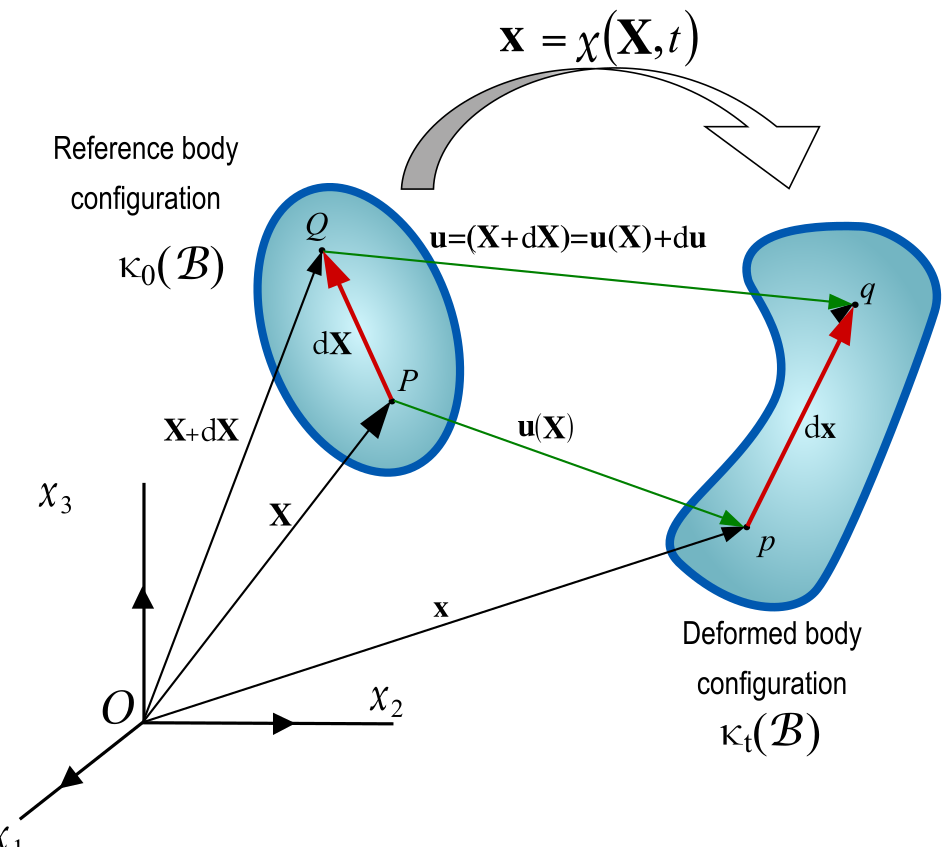
\includegraphics[width=\linewidth]{../Pictures/Continuum_body_deformation}
	\end{column}
	%
	\hfill
	%
	\begin{column}{.6\textwidth}
		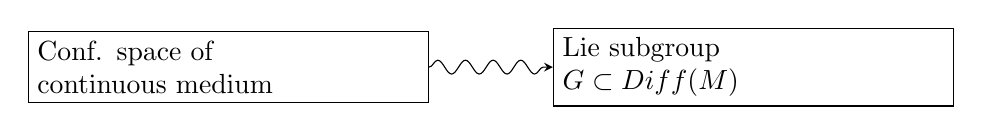
\begin{tikzpicture}[
			text width=0.4\linewidth,
			node distance=0.55\linewidth,
			]
			\node [rectangle,draw] (lhs) {Conf. space of\\ continuous medium};
			\node [rectangle,draw,right of=lhs] (rhs) {Lie subgroup \\$G \subset Diff(M)$};
			\draw[-stealth,decorate,decoration={snake}] (lhs) -- (rhs);
		\end{tikzpicture}

		Examples:
		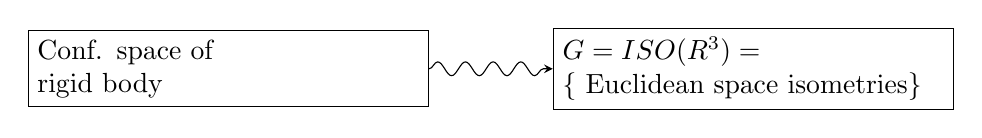
\begin{tikzpicture}[
			text width=0.4\linewidth,
			node distance=0.55\linewidth,
			]
			\node [rectangle,draw] (lhs) {Conf. space of\\ rigid body};
			\node [rectangle,draw,right of=lhs] (rhs) {$G=ISO(\mathbb{R}^3)=$\\ $\{$
				Euclidean space isometries$\}$};
			\draw[-stealth,decorate,decoration={snake}] (lhs) -- (rhs);
		\end{tikzpicture}
		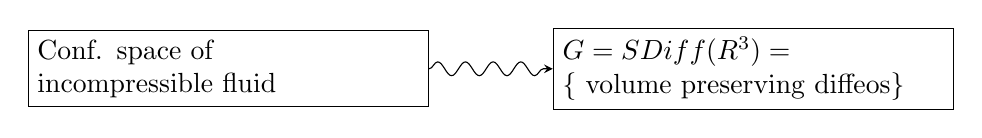
\begin{tikzpicture}[
			text width=0.4\linewidth,
			node distance=0.55\linewidth,
			]
			\node [rectangle,draw] (lhs) {Conf. space of\\ incompressible fluid};
			\node [rectangle,draw,right of=lhs] (rhs) {$G= SDiff(\mathbb{R}^3)=$\\ $\{$
				volume preserving diffeos$\}$};
			\draw[-stealth,decorate,decoration={snake}] (lhs) -- (rhs);
		\end{tikzpicture}
	\end{column}%
	\end{columns}
	\pause
%  	\begin{lemblock}[$(\mathbb{R}^3,\nu = dx\wedge dy\wedge dz)$ is 2-plectic]
%  		\vspace{-2em}
%  		\begin{itemize}
%  			\item \emph{(Easy proof)} 
%  			$\quad \iota_v \nu = \frac{1}{2}\epsilon_{i j k} v^i dx^j \wedge dx^k = 0 \; \Leftrightarrow \; v=0 $;
%  			\item \emph{(Conceptual proof)} 
%  			$\quad \alpha^{(1)} = \ast \circ \flat$ is invertible.
%  		\end{itemize}
%  	\end{lemblock}
	\begin{itemize}[<+->]
		\item Consider the 2-plectic manifold $(\mathbb{R}^3,\nu = dx\wedge dy\wedge dz)$
		\item Consider a subalgebra of the infinitesimal action of $SDiff(\mathbb{R}^3)$:
		  	\begin{displaymath}
		  		\mathfrak{g} = sdiff_0(M) = 
		  		\lbrace  X \in \mathfrak{X} \quad\vert\quad 
		  		div X = 0, \textrm{\emph{ rapidly vanishing at }}\infty \rbrace
		  	\end{displaymath}
		\item \alert{Does this $\infty$-dim. Lie algebra admit an HCMM?}	
	\end{itemize}
  
  \end{frame}
  \note[itemize]{
	%\item  Now we are ready to get to the real business. Namely, give an explicitly construction of a HCMM related to hydrodynamics.
	\item We are working in the setting of \emph{geometric continuum mechanics} .\\
		Recall that the configuration space of a continuum object is encoded via diffeomorphisms. In the case of an incompressible fluid is encoded via volume-preserving diffeomorphisms.
	\item (Configution space is the set of spatial displacement of a mechanical systems. These are different from the \emph{physical states}.
	\item Such manifolds are infinite dimensional. Particular caution has to be taken in defining the smooth structure in this case.
	\item However, what really matters in the construction of a moment map is the infinitesimal action, i.e. the Lie algebra. In our case, the infinitesimal action to be considered is via divergence-free vector fields.
	\item (Notation): In the following M will be the 3 dimensional Euclidean Space.
	\item The simple but crucial observation is that the standard volume form on the euclidean space is a multisymplectic form.
	\item In the following, we will see that the standard Riemannian structure takes a role in our construction. 
	That was the reason to show also a "conceptual proof".
	\item Notation: $\ast = $ and $\sharp = $ are respectively the Hodge operator and the Riemannian sharp operator pertaining to the standard metric in $\mathbb{R}^3$.	
  }
%------------------------------------------------------------------------------------------------

%-------------------------------------------------------------------------------------------------------------------------------------------------
\begin{frame}[fragile]{Results (joint work with M. Spera)}
	\begin{itemize}[<+->]%[<alert@+>]
		\item[\CheckedBox]  Explicit construction of an HCMM for $SDiff_0 \circlearrowright (\mathbb{R}^3,\nu)$ (and generalization to Riemannian homological spheres);
		\item[\CheckedBox]  Hydrodynamics interpretation: proved that this HCMM trasgresses to the standard hydrodynamical co-momentum map of  Arnol'd, Marsden and Weinstein and others;
		% is exhibited upon resorting to the Euler equation for perfect fluids.
		\item[\CheckedBox]  Application to knot theory: reinterpretation of the (Massey) higher order linking numbers in terms of conserved quantities and determined the knot theoretic analogues of first integrals in involution.
	\end{itemize}
	%
	\pause
	\begin{center}
		\includegraphics{beamericonarticle} 
		\textbf{On some (multi)symplectic aspects of link invariants},
		\includegraphics{beamericonarticle} \\ 
		\emph{AMM, Mauro Spera}, \href{https://arXiv.org/abs/1805.01696}{arxiv:1805.01696};\\
		(To appear in \emph{Journal of the Australian Mathematical Society})	
	\end{center}		
	\vfill \pause
	\begin{itemize}
		\item[\CheckedBox]  Aside: a semiclassical interpretation of the HOMFLYPT polynomial.
	\end{itemize}
	%
	\pause
	\begin{center}
		\includegraphics{beamericonarticle} 
		\textbf{Derivation of the HOMFLYPT knot polynomial via helicity and geometric quantization},
		\includegraphics{beamericonarticle} \\ 
		\emph{AMM, Mauro Spera}, \href{https://arxiv.org/abs/1910.13400}{arXiv:1910.13400};\\
		(To appear in \emph{Bollettino dell'Unione Matematica Italiana})	
	\end{center}			
	
\end{frame}
\note[itemize]{
	\item About the explicit construction see frame \ref{frame:explicithcmm} in appendix.
	\item About the hydrodynamical interpretation see frame \ref{frame:hydrointerpretation} 	%\item About the Riemmanian generalization see \ref{frame:riemannianhcmm}
	\item About the application to knots theory see frame \ref{frame:msknots1} and \ref{frame:msknots2} in appendix.
}
%-------------------------------------------------------------------------------------------------------------------------------------------------





%-------------------------------------------------------------------------------------------------------------------------------------------------
\subsubsection{JW Leonid}
%-------------------------------------------------------------------------------------------------------------------------------------------------
	\begin{frame}{Results}
		\begin{columns}[T]
			\begin{column}{0.3\textwidth}
				\centering
					\fbox{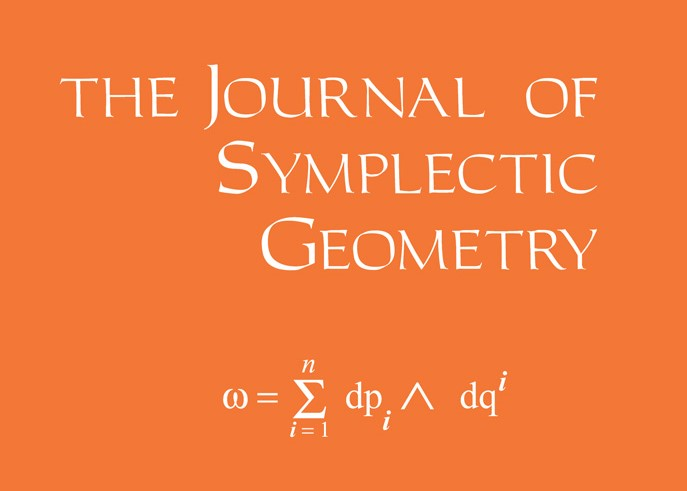
\includegraphics[width=.9\textwidth]{./Pictures/cover-JSG}}

			\end{column}		
			\begin{column}{0.7\textwidth}
				\begin{itemize}
					\item[-] Complete classification of Hamiltonian actions on spheres (multisymplectic w.r.t. the canonical volume form).
					\item[-] Explicit expression of momenta for $SO(n)\circlearrowleft S^n$ and other cases.
				\end{itemize}
			\end{column}		
		\end{columns}				
\end{frame}
%---------------------------------------------------------------------------------------------------------------------------------------------------

%-------------------------------------------------------------------------------------------------------------------------------------------------
\begin{frame}[fragile]{Cohomological obstruction to HCMM}
A HCMM is a sequence of linear maps:
			\begin{displaymath}
				(f)  = \big\lbrace f_k: \; \Lambda^k{\mathfrak g} \to L_{k-1} \subseteq \Omega^{n-k} 
				\;\big\vert\; 0\leq k \leq n+1  \big\rbrace
			\end{displaymath}
it can be interpreted as a primitive of a certain cocycle in the total complex of 
	\begin{displaymath}
		(C_\mathfrak{g}^{\bullet,\bullet} = \Lambda^{\geq 1} 
		\mathfrak{g}^*\otimes \Omega^\bullet(M), \delta_\text{CE},d),	
	\end{displaymath}
	%
	\pause
	\begin{propblock}[$\exists$ HCMM 
		$\Leftrightarrow ~ \lbrack\tilde{\omega}\rbrack=0\in H^{n+1}(C_\mathfrak g^\bullet,d_ {tot})$	
	]
		\begin{columns}
		\begin{column}{.5\textwidth}
			\begin{displaymath}
				\tilde{\omega} = \sum_{k=1}^{n+1} (-1)^{k-1} \iota^k_\mathfrak{g} \omega \in C_\mathfrak{g}^{n+1},
			\end{displaymath}		
		\end{column}
		\begin{column}{.5\textwidth}
			\begin{align*}
				\iota^k_\mathfrak{g} \colon \Omega^\bullet(M)
				&\to \Lambda^k \mathfrak{g}^\ast \otimes \Omega^{\bullet-k}(M)
				\\ \omega&\mapsto \omega_k = 
				\left(p \mapsto \iota_{v_p} \omega  \right) ,
			\end{align*}
		\end{column}		
		\end{columns} 
	\end{propblock}
	%
	\pause
	\begin{corblock}[Cohomological condition for $\vartheta:G\times M\to M$ compact Lie group action]
	$$\exists \text{ HCMM} 
		\Leftrightarrow ~[\vartheta^*\omega-\pi^*\omega]=0\in H^{n+1}(G\times M)$$ 
	\end{corblock}

\end{frame}
\note[itemize]{
	\item 
	The  corresponding total complex is given by
	\begin{displaymath}
		(C_\mathfrak{g}^{\bullet}, d_\text{tot} = 
		\delta_\text{CE}\otimes \text{id} + \text{id}\otimes d),
	\end{displaymath}
	where $d$ denotes the de Rham differential and $\delta_{CE}:\Lambda^k\mathfrak g^*\to \Lambda^{k+1}\mathfrak g^*$ the Lie algebra cohomology differential.
	According to the Koszul sign convention, $d_{\text{tot}}$ acts on an element of $\Lambda^k \mathfrak{g}^*\otimes \Omega^\bullet(M)$ as $\delta_\text{CE} + (-1)^k d$.

	\item PROP: the primitives of the natural cocycle $\tilde{\omega}$ are in one-to-one correspondence with comoments of $v$.
	
	\item COR: Let $\vartheta:G\times M\to M$ be a compact Lie group acting on a pre-multisymplectic manifold, preserving the pre-multisymplectic form $\omega$. 
A comoment exists if and only if $[\vartheta^*\omega-\pi^*\omega]=0\in H^{n+1}(G\times M)$.
	\item Note that here we employ the deRham cohomology of the product. This is different from the equivariant cohomology
	\item some more details in \ref{frame:cohomologicalproposition} of the appendix.
}
%-------------------------------------------------------------------------------------------------------------------------------------------------


%-------------------------------------------------------------------------------------------------------------------------------------------------
\begin{frame}[fragile]{Results (Joint work with L. Ryvkin)}
	Let $G\times M\to M$ be a compact Lie group preserving a pre-multisymplectic form $\omega$.
	\begin{itemize}
		\item[\CheckedBox]  Proved, without resorting on a specific model, that if $[\omega]\in H^\bullet(M)$ lies in the image of $q^*:H^\bullet_G(M)\to H^\bullet(M)$, then $\vartheta$ admits a comoment.
	\end{itemize}
	%\noindent\makebox[\linewidth]{\rule{\paperwidth}{0.4pt}}
	\pause
	\vspace{1em}
	Consider now $(M,\omega)$ to be a $n$-dimensional sphere together with the standard volume:
	%
			\begin{claimblock}
				Let $\vartheta:G\times S^n \to S^n$ be an effective,compact multisymplectic action,
				\begin{center}
					$\vartheta$ admits HCMM $~\Leftrightarrow~$ $n$ is even or $\vartheta$ is not transitive.
				\end{center}
			\end{claimblock}
	%
	\begin{itemize}
		\item[\CheckedBox]  	Explicit construction for 
	$SO(n)~\circlearrowleft~S^{n}$ and
	$G_2~\circlearrowleft~(S^6,\phi)$
		\item[\CheckedBox]   Explicit expression for the first 2 components of HCMM for 
			$SO(n+1)~\circlearrowleft~S^{n}$.
		 (Going higher can be set up as a computational problem. We sketched a prototype code in python.)
		 	\end{itemize}

	\pause
	\begin{center}
		\includegraphics{beamericonarticle} 
		\textbf{Multisymplectic actions of compact Lie groups on spheres},
		\includegraphics{beamericonarticle} \\ 
		\emph{AMM, Leonid Ryvkin}, \href{https://arxiv.org/abs/1906.08790}{arXiv:1906.08790};\\
		(To appear in \emph{Journal of Symplectic Geometry})	
	\end{center}		


\end{frame}
\note[itemize]{
	\item 	Let a compact Lie group $G$ act on a manifold $M$. Let $EG$ be a contractible space on which $G$ acts freely by $\vartheta^{EG}$. Then we define the equivariant cohomology of $M$ as $H^\bullet_G(M):=H^\bullet((M\times EG)/G)$, where $G$ acts on $M\times EG$ diagonally.

	\item As $EG$ might not be a manifold, we have to interpret $H^\bullet(\cdot)$ as a suituable cohomology theory (e.g. singular cohomology with real coefficients) in the above definition.
	
	\item As $G$ is compact, when $\vartheta:G\times M\to M$ is a free action, we have $H_G^\bullet(M)=H^\bullet_{dR}(M/G)$. For a not necessarily free action $\vartheta$, we still have the following diagram
	$$
		G\times (M\times EG) \xrightarrow{\vartheta\times \vartheta^{EG}}
		M\times EG \xrightarrow{q} (M\times EG)/G
	$$
	where $q$ is the projection to the orbits, which induces $q^*$ in cohomology.

	\item We gave	an intrinsic proof of Theorem which does not depend on the choice of a model for equivariant cohomology. 
	
	\item	
	Unlike the symplectic case, the converse statement does not hold in general. 
	Even if a (pre-)multisymplectic action of $G$ on $(M,\omega)$ admits a comoment, $[\omega]$ does not need to come from an equivariant cocycle. 
	
	\item 	
	First 2 component of HCMM for $SO(n+1)$ on $S^{n}$ (Going higher can be set up as a computational problem - we have a sketch of code in Python -, the first 2 component are easier due to the vanishing of the first two CE cohomology group of $G$)
}
%-------------------------------------------------------------------------------------------------------------------------------------------------



%-------------------------------------------------------------------------------------------------------------------------------------------------
\subsubsection{JW Marco}
%-------------------------------------------------------------------------------------------------------------------------------------------------
	\begin{frame}{Results}
		\begin{columns}[T]
			\begin{column}{0.3\textwidth}
				\centering
					\fbox{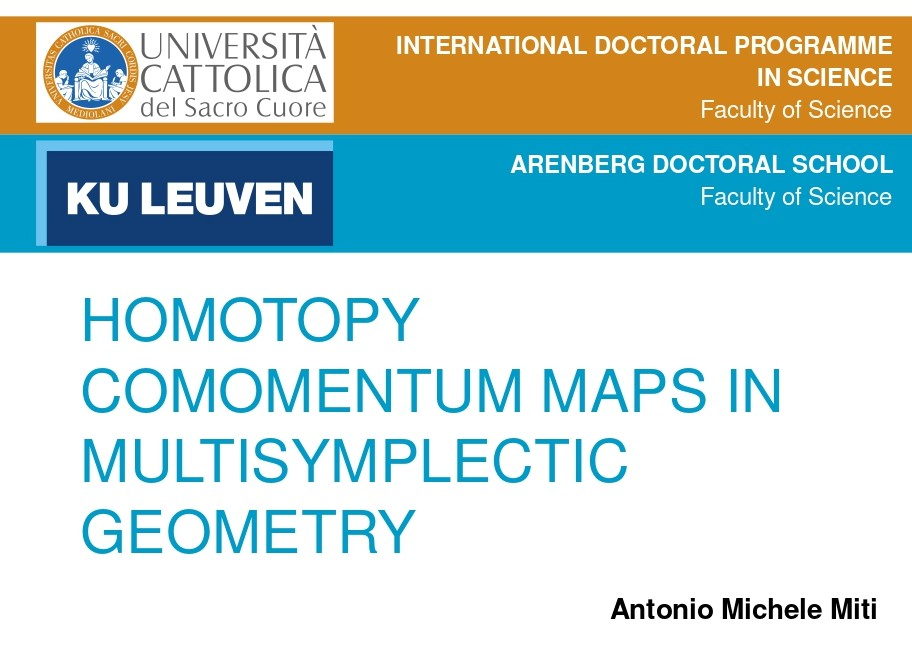
\includegraphics[width=.9\textwidth]{./Pictures/cover-Thesis}}
					
					\vspace{1em}
					\fbox{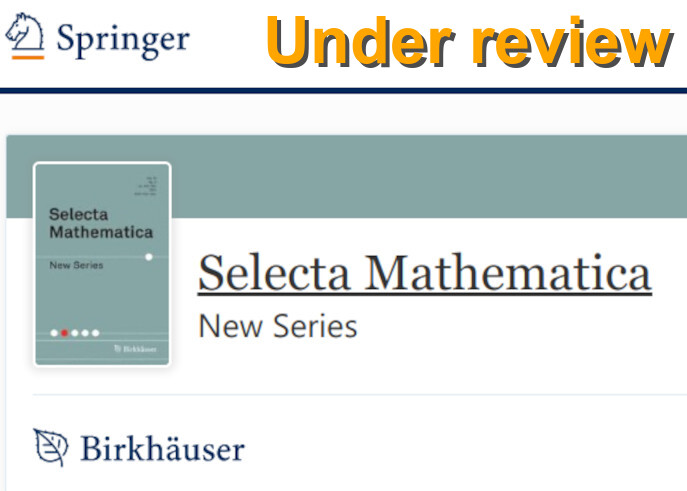
\includegraphics[width=.9\textwidth]{./Pictures/cover-Selecta-honest}}
			\end{column}		
			\begin{column}{0.7\textwidth}
				\begin{itemize}
					\item<1->[-] Compatibility of \emph{Homotopy comomentum maps} w.r.t. gauge-related multisymplectic manifolds.
					\item<1->[-] Relationship between the $L_\infty$-algebra of observables and \emph{higher courant algebroids.} 				
				\end{itemize}	
			\end{column}		
		\end{columns}
\end{frame}
%---------------------------------------------------------------------------------------------------------------------------------------------------
\begin{frame}[fragile]{Relation to higher Courant algebroids (Joint with M. Zambon)}
	%
	Consider $(M,\omega)$ \alert{symplectic mfd.}
	\only<3-11>{ and \alert{prequantizable} ($S^1$-bundle $P$, connection $\theta$)}
	\vfill
	\includestandalone[width=\textwidth]{../Pictures/Frame_BigDiagram_symplectic}
	%
	\begin{minipage}[t][2cm][t]{\textwidth}
	\begin{itemize}
		\only<1-6>{
			\item<2-> Given a Symp. mfd. $(M,\omega)$ there is a naturally associated Poisson algebra ...
			\item<4-> .\alert<+>{... and also a Lie Algebroid}.
			\item<5-> A Lie algebroid is a "controlled" $\infty$-dimensional Lie algebra;
		}
		\only<7-11>{
		\item<7-> Consider a deformed structure $\tilde{\omega}= \omega + d B$ with $B\in C^\infty(M)$;
		\item<9-> There is a natural isomorphism in the Lie Alg.oids category,
		\item<11-> Considering $\mathfrak{g}\circlearrowleft M$ preserving $\omega$ and $\tilde{\omega}$ ...
		}
		\item<12-> Neglect the prequantization...
		\vspace{-1em} 
			\begin{displaymath}
				\begin{tikzcd}
					\Psi~:&[-1em] C^{\infty}(M)_\omega \ar[r,"\Psi"]& \Gamma(TM\oplus \mathbb{R})_\omega
					\\[-2em]
					& f \ar[r,mapsto] & \binom{\mathscr{v}_f}{f}
				\end{tikzcd}
			\end{displaymath}
	\end{itemize}
	\end{minipage}
	\vfill
	\tcbset{colback=white,
	colbacktitle=white,
	colframe=red!70!black,
	boxrule=1pt,
	colupper=red!70!black,
	arc=15pt,
	}
	\begin{minipage}[t][2cm][t]{\textwidth}
	\only<6>{ 
		\begin{tcolorbox}
			There is a natural embedding $C^\infty \to \Gamma(TM\oplus\mathbb{R})$\\
			\underline{independent from the prequantization $(P,\theta)$}.
		\end{tcolorbox}
	}
	\only<11>{ 
		\begin{tcolorbox}
			\centering The central diagram commutes!
		\end{tcolorbox}
	}
	\only<12>{
		\begin{tcolorbox}	
			\centering The central pentagon commutes!
		\end{tcolorbox}	
		
	\begin{center}
		\alert{
		\faQuestionCircle \qquad
			{What happens in the higher (n-plectic) case?}	
		\qquad \faQuestionCircle		
		}
	\end{center}		
		
	}
	\end{minipage}
	%
\end{frame}
\note[itemize]{
	\item The horizontal embedding is  $f \mapsto (v_f,f)$;
	\item Vertical maps are also known as \emph{Gauge transformations}
}
%-------------------------------------------------------------------------------------------------------------------------------------------------

%-------------------------------------------------------------------------------------------------------------------------------------------------
\begin{frame}{Relation to higher Courant algebroids (Joint with M. Zambon)}
	Consider now $\omega$ \alert{multisymplectic}
	\vfill
	%
	\includestandalone[width=\textwidth]{../Pictures/Frame_BigDiagram_k-plectic}
	%
	\vfill
	%
	
	\onslide<1->{
	\begin{itemize}
		\item<3-> Higher analogue of the Courant algebroid $\rightsquigarrow$ \emph{Vinogradov algebroid} $\mathbb{T}M =(TM\oplus\bigwedge^{k-1}T^\ast M)$
		\item<4->  Vin. alg.oids are $NQ$-manifolds, there's associated $L_\infty$-algebra
	\end{itemize}
	
	
	}
	\vfill
	\tcbset{colback=white,
		colbacktitle=white,
		colframe=blue!70!black,
		boxrule=1pt,
		colupper=blue!70!black,
		arc=15pt,
		}
	\onslide<5->{
	\begin{tcolorbox}[sidebyside,righthand width=.75\linewidth]
		Thm: \cite{Miti2021}
		\tcblower
		\begin{itemize}
			\item<.-|alert@.>
				There is an embedding of $L_\infty$-algebras  $L_\infty(M,\omega)\hookrightarrow L_{\infty}(\mathbb{T}M,\omega)$.
			\item<8-|alert@+> The central square commutes.
		\end{itemize}
	\end{tcolorbox}	}
	

\end{frame}
\note[itemize]{
	\item Our results can be seen as a tiny step toward  undestanding the analogue of prequantization in the setting of multisymplectic geometry (hence field theory).
}
%-------------------------------------------------------------------------------------------------------------------------------------------------



%-------------------------------------------------------------------------------------------------------------------------------------------------
\subsubsection{JW LeoCas}
%-------------------------------------------------------------------------------------------------------------------------------------------------
	\begin{frame}{Results}
		\begin{columns}[T]
			\begin{column}{0.3\textwidth}
				\centering
					\fbox{
\includegraphics[width=.9\textwidth]{./Pictures/cover-PJM-honest}}
			\end{column}		
			\begin{column}{0.7\textwidth}
				\begin{itemize}
					\item<1->[-] .
					\item<1->[-] .			
				\end{itemize}	
			\end{column}		
		\end{columns}
		\vfill
\end{frame}
%---------------------------------------------------------------------------------------------------------------------------------------------------


%-------------------------------------------------------------------------------------------------------------------------------------------------
\begin{frame}{Singular Reduction: Roadmap}
	%
	\begin{block}{Data:}
			\begin{itemize}
				\item A \emph{constraint set} $N$ (possibly singular),
				\item An infinitesimal action preserving $N$.
			\end{itemize}
	\end{block}
	%
	\vfill
	\pause
	%
	\begin{block}{Goal:}
		\begin{itemize}
			\item Obtain a "reduced" observables algebra out of the data.
		\end{itemize}
	\end{block}
	%
	\vfill
	\pause
	%
	\begin{block}{Strategy:}
		\begin{enumerate}
			\item Define smooth fields/forms \emph{tangent to $N$},
			\item define smooth fields/forms \emph{vanishing along $N$},
			\item define \emph{reducible fields} requiring the preservation of the vanishing objects,
			\item define \emph{reducible forms} requiring their conservation w.r.t. the infinitesimal action,
			\item define \emph{reducible and vanishing observables},
			\item \textbf{quotient}
		\end{enumerate}
	\end{block}






\end{frame}

%-------------------------------------------------------------------------------------------------------------------------------------------------


%-------------------------------------------------------------------------------------------------------------------------------------------------
\begin{frame}[shrink]{Smooth objects on a singular set}
	Consider $N$ closed subset of $M$.
	\vfill
	\pause
	\begin{defblock}
	 $I_N$ = ideal of smooth functions vanishing over $N$.
	\end{defblock}
	\vfill
	\pause

	\begin{columns}[T]
		\setlength{\belowdisplayskip}{5pt}
		\begin{column}{.65\linewidth}
			%
			\centering \it
				\begin{defblock}[v.f tangent to $N$]
					\begin{displaymath}
						\X_N(M):=
						\left\lbrace
							v \in \X(M)
						~\Big\vert~
							\L_v(I_N) \subseteq I_N
						\right\rbrace
					\end{displaymath}
				\end{defblock}
				\begin{defblock}[v.f vanishing on $N$]
					\begin{displaymath}
						I_\X(N):=
						\left\lbrace
							v \in \X(M)
						~\Big\vert~
							\L_v(C^\infty(M)) \subseteq I_N
						\right\rbrace
					\end{displaymath}				
				\end{defblock}				
		\end{column}	
		%
		%
		\begin{column}{.35\linewidth}
			\centering 
			\includestandalone[width=0.8\textwidth]{Pictures/Figure_VfTangentN}			
		\end{column}	
	\end{columns}			
	%	
	\pause

				%

				%	
		\begin{tcolorbox}[
		enhanced,frame hidden,borderline={0.5pt}{0pt}{blue},
		arc=5pt,colback=white,
		colbacktitle=white,]
			\color{blue}{\textbf{Lem}:} If $N$ is smoothly embedded,  $\X(N)\cong {X_N(M)}/{I_\X}$.
		\end{tcolorbox}

		\pause

		\begin{defblock}[Differential form vanishing on $N$]
			\begin{displaymath}
				I_{\Omega(N)}:=
				\left\lbrace
					\alpha\in\Omega^k(M
				~\left\vert~
					\begin{array}{l r}
						k\geq 0,~		\\		
						\alpha(u_1,\ldots,u_k) \in I_N & \forall u_i \in\X_N(M)
					\end{array}
				\right\rbrace\right.
			\end{displaymath}
		\end{defblock}

\end{frame}
\note[itemize]{
 \item $N$ is not a submanifold in general. An example is $N=\mu^{-1}(0)$ for a certain smooth map $N$.
 \item observe that if $N$ is a smooth embedded submanifold, one has that $\X(N)\cong \frac{X_N(M)}{I_\X}$  

}
%-------------------------------------------------------------------------------------------------------------------------------------------------



%-------------------------------------------------------------------------------------------------------------------------------------------------
\subsection{Multisymplectic singular reduction}
\begin{frame}{Reducible smooth objects \quad \small (w.r.t. $N$ and $\g\action M$)}
	Consider $\g \action M$ by vector fields tangent to $N$ % \hfill( fond. distribution $\underline{\g}\subseteq \X_N(M)$)
	\\
	\vfill
	Denote by :  
	\hspace{1em} $\underline{\g}\subseteq \X_N(M)$ the fundamental distribution,
	\\
	\hspace{6.5em}  $\X_g$ the $C^\infty$-module generated by $\underline{\g}$.
	\\
	\vfill
	\begin{defblock}[Reducible v.fields ]
			\begin{displaymath}
				\X(M)_{[N]} :=
				\left\lbrace
					v \in \X(M)
				~\left\vert~
					\begin{array}{l}
						\L_v (I_N) \subseteq I_N	\\		
						\L_v (\X_g) \subseteq \X_g + I_\X
					\end{array}
				\right\rbrace\right.
			\end{displaymath}
%			\blfootnote{
%			 $\X_g$ = $C^\infty(M)$-module generated by the fundamental distribution.
%			}	

	\end{defblock}	
	%
	\pause
	%
	\begin{defblock}[Reducible forms ]
		\begin{displaymath}
			\Omega(M)_{[N]} :=
			\left\lbrace
				\alpha \in \Omega(M)
			~\left\vert~
				\begin{array}{l r}
					\L_\underline{\xi} \,\alpha \in I_{\Omega(N)}	\\		
					\iota_\underline{\xi} \,\alpha \in I_{\Omega(N)}	& \forall \xi \in \g				\end{array}
			\right\rbrace\right.
		\end{displaymath}	
	\end{defblock}	
	%
	\pause
	%
	\begin{defblock}[Reducible Hamiltonian forms]
		\begin{displaymath}
			(\Omega(M)_{ham}^{n-1})_{[N]} :=
			\left\lbrace
				\alpha \in \Omega(M)_{ham}^{n-1}
			~\left\vert~
				\begin{array}{l r}
					\alpha \text{ is a reducible form} \\
					\vHam_\alpha \text{ is a reducible v.field}
				\end{array}
			\right\rbrace\right.
		\end{displaymath}	
	\end{defblock}		

	
\end{frame}
\note[itemize]{
 \item $\g\action M$ by vector field tangent to $N$ means that $\underline{\xi}\in\X_n(M) \forall \xi \in \g$
 \item Spelling out the definition: reducible vector fields are 
 \\i) v.f. tangent to N 
 \\ii) such that their commutator with any $\underline{\xi}$ lies in $\X_\g$ along $N$.
 \item more algebraically, they stabilize both $I_N$ and $\X_g + I_\X$.
 \item observe that $\L_v I_\X \subseteq I_\X$ since , $\forall u \in I_\X$ $\forall f \in C^\infty(M)$ one has\\
 $(\L_v u) f = \L_{[v,u]} f = \L_v\L_u f - \L_u\L_v f \in I_N$
 \item
}
%-------------------------------------------------------------------------------------------------------------------------------------------------

%-------------------------------------------------------------------------------------------------------------------------------------------------
\begin{frame}{Singular reduction}
	\begin{defpropblock}[Reducible $L_\infty$-observables]
		Is the {\color{blue!70!black}$L_\infty$-subalgebra} of $L_\infty(M,\omega)$ given by
		\begin{displaymath}
			L_\infty(M,\omega)_{[N]}^k :=
			\begin{cases}
				\Omega^{n-1-k}(M)_{[N]} 
				\qquad\text{\color{gray}\small (reducible forms) }
				& \text{if } n-1\leq k < 0 \\
				(\Omega(M)_{ham}^{n-1})_{[N]} 
				\quad
				\text{\color{gray}\small (reducible hamiltonians) }
				& \text{if } k = 0 \\
				0 & \text{if } k > 0
			\end{cases}
		\end{displaymath}
	\end{defpropblock}
	%
	\pause
	%
	\begin{defpropblock}[Vanishing $L_\infty$-observables]
		Is the {\color{blue!70!black}$L_\infty$-ideal} of $L_\infty(M,\omega)_{[N]}$ given by
		\begin{displaymath}
			I_{L_\infty(M,\omega)} :=
			\left\lbrace
				\alpha \in L_\infty(M,\omega)_{[N]}
			~\left\vert~
				\begin{array}{l l}
					\alpha(v_1,\dots,v_k) \in I_N  \quad \forall v_i \in \X_N &
					\text{if}~ \alpha \in \Omega^k \\
					\vHam_\alpha \in \X_\g + I_\X &
					\text{if}~ \alpha \in \Omega^{n-1}
				\end{array}
			\right\rbrace\right.
		\end{displaymath}
	\end{defpropblock}
	%
	\pause
	%
	\begin{defblock}[Reduced $L_\infty$-algebra of observables]
		Is the $L_\infty$-quotient : \quad
		$\dfrac{L_\infty(M,\omega)_{[N]}^k}{I_{L_\infty(M,\omega)}}$
	\end{defblock}

\end{frame}
\note[itemize]{
 \item The graded vector space underlying the reduced $L_\infty$-algebra $\Ham_\infty(M,\omega)_N$ is explicitly given by
\begin{displaymath}
	\Ham_\infty(M,\omega)_N =
	\frac{
		\left\lbrace
			(\alpha,v) \in \Omega(M){[n{-}1]}\oplus\X(M)
		~\left\vert~
			\begin{array}{l l}
				\iota_v \omega = -\d \alpha^{(0)} &
				\\
				\iota_\xi \alpha \in I_{\Omega}(N) &
				\\
				\L_\xi\alpha \in I_{\Omega}(N)
				&
				\\
				\L_\xi v \in \fgmodule +\vanvf
				&~\forall \xi \in \g 
				\\
				v \in \X_N(M)
				&
			\end{array}
		\right.
		\right\rbrace
	}{
		\left\lbrace
			(\alpha,v) \in \Omega(M){[n{-}1]}\oplus\X(M)
		~\left\vert~
			\begin{array}{l}
				\alpha \in I_{\Omega}(N)
				\\
				v \in \fgmodule +\vanvf
			\end{array}
		\right.
		\right\rbrace
	}~.
\end{displaymath}
}
%-------------------------------------------------------------------------------------------------------------------------------------------------

%-------------------------------------------------------------------------------------------------------------------------------------------------
\begin{frame}{Singular reduction (Upshot and conclusions)}

	\begin{itemize}
		\item Consider $N=\mu^{-1}(0)$ to be regular (smooth embedding)
		\vspace{.5em}
		\begin{table}[]
			\begin{tabular}{ccc}
			Multisymplectic               &                      & Multisymplectic                  \\
			regular                       & $\equiv$             & singular                \\
			reduction & & reduction
			\end{tabular}
		\end{table}	
		
		\pause
		\item
			Consider $\omega$ to be $1$-plectic
			\vspace{.5em}
			\begin{table}[]
				\begin{tabular}{ccc}
				Multisymplectic               &                      &  Sniaticky--Weinstein                  \\
				singular                       & $\cancel\equiv$             & singular                \\
				reduction & & reduction
				\end{tabular}
			\end{table}	

			(but $\exists$ a canonical Poisson algebra morphism)
	\end{itemize}
	
	\pause
			\vfill
		  \centering 
		  {\Huge\color{red} 
		  \emph{Thank you for your attention!}}
			\vfill
\end{frame}
\note[itemize]{
 \item
}
%-------------------------------------------------------------------------------------------------------------------------------------------------





%-------------------------------------------------------------------------------------------------------------------------------------------------
\section{Research Proposal}
\subsection{Ongoing projects}
\checkpoint
%-------------------------------------------------------------------------------------------------------------------------------------------------

%-------------------------------------------------------------------------------------------------------------------------------------------------
\begin{frame}{Observables quantities in multisymplectic geometry}

\end{frame}
\note[itemize]{
	\item  Research Line A

}
%-------------------------------------------------------------------------------------------------------------------------------------------------

%-------------------------------------------------------------------------------------------------------------------------------------------------
\begin{frame}{Reduction commutes with Prequantization}

\end{frame}
\note[itemize]{
	\item  Research Line B

}
%-------------------------------------------------------------------------------------------------------------------------------------------------

%-------------------------------------------------------------------------------------------------------------------------------------------------
\begin{frame}{Multisymplectic PDEs and Integrators}

\end{frame}
\note[itemize]{
	\item  Research Line C

}
%-------------------------------------------------------------------------------------------------------------------------------------------------


%-------------------------------------------------------------------------------------------------------------------------------------------------
\begin{frame}{Open questions on covariant observables (Preliminary)}
	%
	\begin{columns}
		%
		\begin{column}{.50\linewidth}
			\begin{center}
				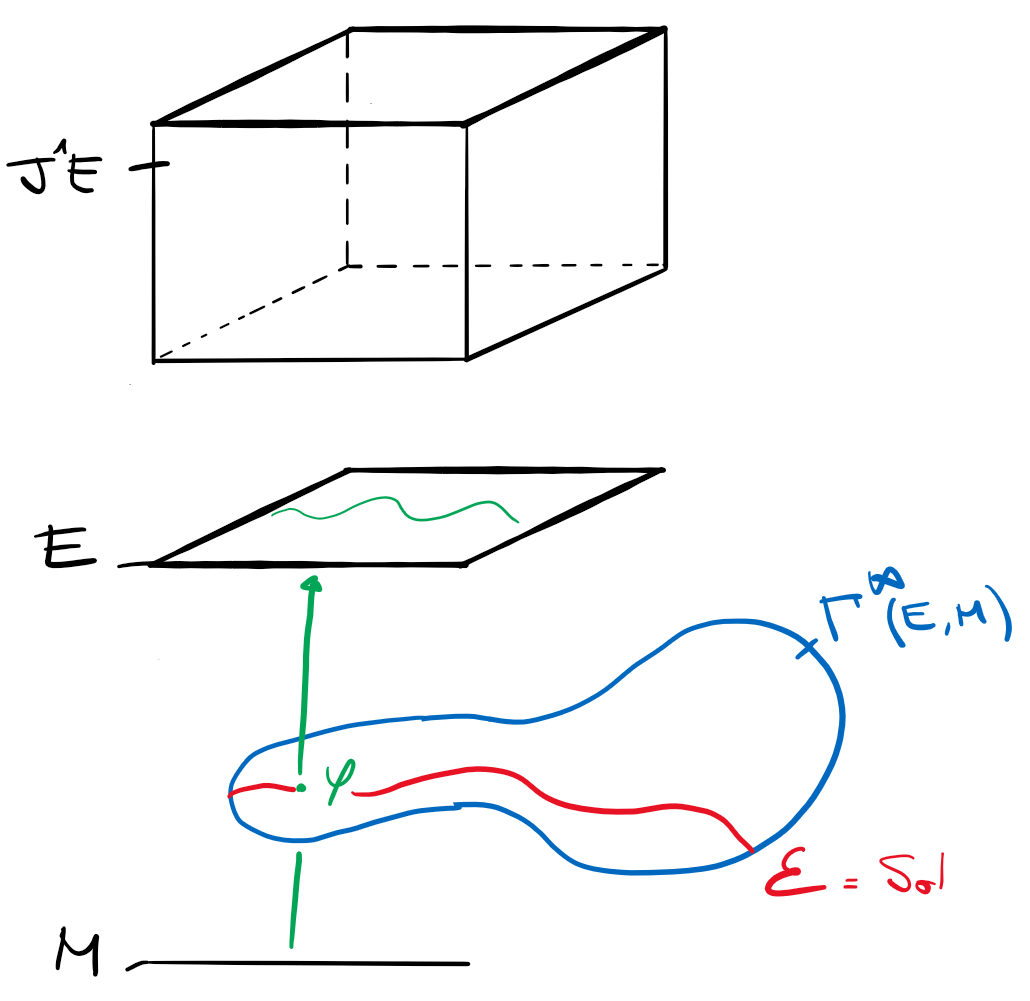
\includegraphics[width=0.9\linewidth]{../Pictures/Covariant}			
			\end{center}
		\end{column}
		%
		\begin{column}{.50\linewidth}
			\begin{itemize}
				\item Consider a classical field $E\to M$ with I-order Lagrangian $\mathcal{L}$;
				\item<2-> $\mathcal{L}$ determines  
					\begin{itemize}
						\item[(a)] a multisymplectic structure on $J^1 E$,
						\item[(b)] a symplectic \emph{Diffiety} $(\mathcal{E})$ called \emph{Covariant phase space}\footnote{Suppose E-L operator being \emph{formally integrable}};
					\end{itemize}
				\item<3-> two different candidates for the role of \emph{physical observables}:
					\begin{itemize}
						\item[(a)] Lie infinity algebra $L_\infty (M,\omega)$;
						\item[(b)] Cochain complex $\bar{\Omega}^\bullet(\mathcal{E})$.
					\end{itemize}
				\item<4-> Questions:
					\begin{itemize}
						\item[-] What is their mutual relationship?
						\item[-] Application to \emph{Multisymplectic PDEs}?
						\item[-] Third actor: the \emph{Space of initial datas}.
					\end{itemize}																		
			\end{itemize}
		\end{column}
		%
	\end{columns}
\end{frame}
\note[itemize]{
	\item the two framework yields different candidates to the role of \emph{physical observable}:
	\item Note that in the classical ordinary case the space of initial data coincides with the phase space

}
%-------------------------------------------------------------------------------------------------------------------------------------------------


%---------------------------------------------------------------------------------------------------------------------------------------------------
\begin{frame}{Research proposal context: (multi)symplectic reduction}
	\textbf{\color{UniGreen}Symplectic reduction:}~~
	Procedure associating to any (suitably regular) pair of symplectic manifold and Hamiltonian action another symplectic manifold of smaller dimension.
	\vfill
	\pause
	\begin{thmblock}[Marsden-Weinstein reduction]
		\vspace{-.4em}
		\begin{tabular}{l p{12cm}}
		    Given: & $(M,\omega)$ symplectic
		    \\
		    & $G\curvearrowright M$ symplectic with equivariant momap. $J:M\to \mathfrak{g}^*$
		    \\[.2em]
		    Assume: & $\mu \in \mathfrak{g}^*$ regular value of $J$ 
		    \qquad\quad \footnotesize \textcolor{gray}{($\Rightarrow$ $J^{-1}(\mu)\hookrightarrow M$ smooth embedding)}
		    \\
			& $G_\mu\action J^{-1}(\mu)$ free and proper
			\quad \footnotesize \textcolor{gray}{($\Rightarrow$ $J^{-1}(\mu)/G_\mu$ smooth manifold)}
			\\[.4em]
			Then: & $\exists!$ symplectic structure $\omega_\mu$ in $M_\mu:= J^{-1}(\mu)/G_\mu$ \\
			& s.t. $\pi^\ast \omega_\mu = j^\ast \omega$ with $j:M_\mu \hookrightarrow M$ and $\pi:M\twoheadrightarrow M_\mu$
		\end{tabular}
		\vspace{-.4em}
	\end{thmblock}
	%
	\vfill
	\pause
	\begin{columns}
		\begin{column}{0.40\textwidth}
			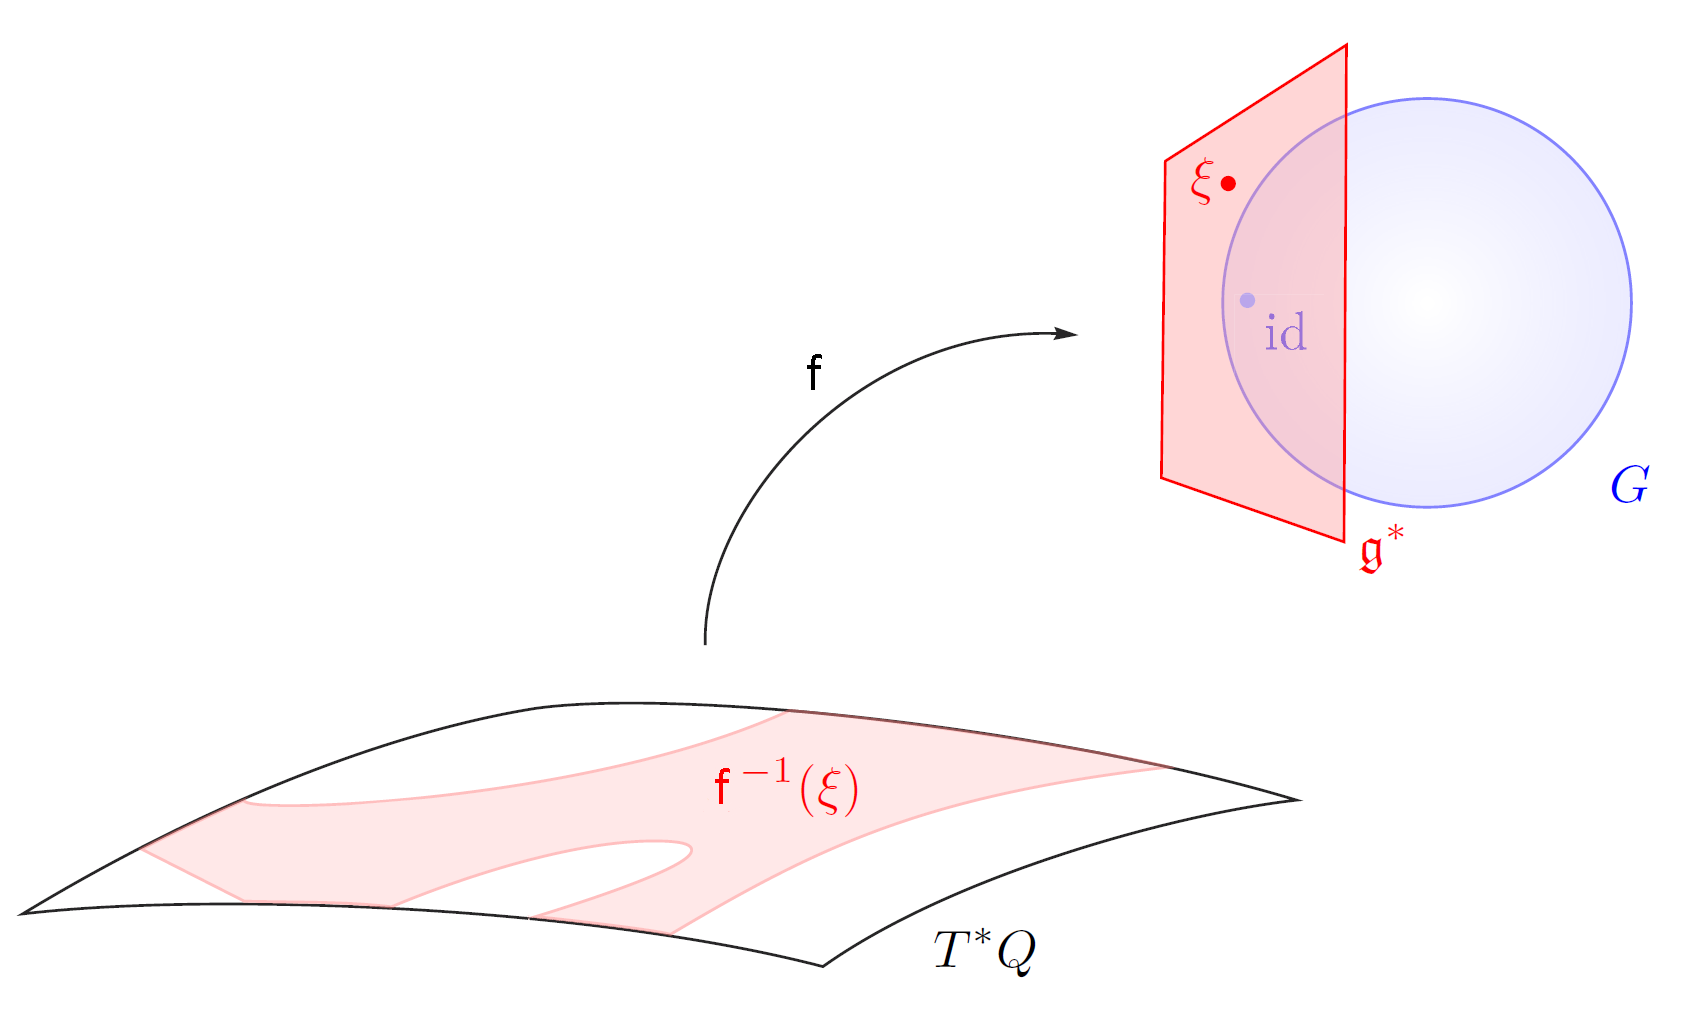
\includegraphics[width=\textwidth]{./Pictures/Reduction}
		\end{column}	
		
		\begin{column}{0.6\textwidth}
				\textbf{\color{UniGreen}In mechanics:}~~
			it embodies the process of restricting the dynamics of the system to the level sets of the conserved quantities pertaining to the symmetry group.		
			\\
			\color{gray}\small( e.g. restricting to studying a point-like particle in a central potential by studying it in radial coordinates only)
		\end{column}	
	\end{columns}	


<\end{frame}
%---------------------------------------------------------------------------------------------------------------------------------------------------


%---------------------------------------------------------------------------------------------------------------------------------------------------
\begin{frame}{Research goals (2022-2023)}
  	%
	\begin{probox}[colback=white]{Multisymplectic regular reduction}
		\begin{itemize}
			\item[\cmark] Recent definition by Blacker:
			\item[\smark] it involves a different notion of \emph{observables};
			\item[\smark] reconcile with the $L_\infty$/homotopy framework.
		\end{itemize}
	\end{probox}
	
	\pause
	\begin{probox}[]{Multisymplectic singular reduction}
		\begin{itemize}
			\item[\cmark] On-going collaboration with Blacker and Ryvkin:
			\item[\smark] complete comparison with other known reduction schemes;
			\item[\smark] higher analogue of \emph{cotangent reduction} theorems;
			\item[\smark] relevant examples.
		\end{itemize}
	\end{probox}

 	\pause
	\begin{probox}[colback=white]{Geometric mechanics perspective}
		\begin{itemize}
			\item[\cmark] MS. geometry stemmed from a geometric formulation of classical field theories:
			\item[\smark] modern development yet to be %fruitfully
			reconciled with physics;
			\item[\smark] reduction of scalar field w.r.t. Poincarè yields the usual field momenta?
			\item[\smark] Streamlined procedure to retrieve ordinary field observables from the multisym. framework.
		\end{itemize}
	\end{probox}  

	\pause
	\begin{probox}[colbacktitle=yellow!15!white ,colback=yellow!15!white]{{[Reduction, Quantization]=0} ?}
		\begin{itemize}
			\item[\cmark] Preliminary results on $2$-plectic prequantization due to Sevestre and Wurzbacher:
			\item[\smark] Investigate compatibility of reduction and prequantization schemes in the multisym. framework.
		\end{itemize}
	\end{probox}	
\end{frame}
%---------------------------------------------------------------------------------------------------------------------------------------------------


%------------------------------------------------------------------------------------------------
% Thank you! slide
%-------------------------------------------------------------------------------------------------------------------------------------------------
	\begin{frame}{}
		\vfill
	  \centering 
	  {\Huge\color{red} 
	  \emph{Thank you for your attention!}}
		\vfill
		%
		\centering
		\begin{columns}
			\hfill
			\begin{column}{0.05\linewidth}
				\centering \includegraphics{beamericonarticle}
			\end{column}
			\begin{column}{0.8\linewidth}
				\centering
				\textbf{On some (multi)symplectic aspects of link invariants},
				\\
				\emph{AMM, Mauro Spera}, \href{https://arXiv.org/abs/1805.01696}{arxiv:1805.01696};\\
				(To appear in \emph{Journal of the Australian Mathematical Society})	
			\end{column}
			\begin{column}{0.05\linewidth}
				\centering \includegraphics{beamericonarticle}			
			\end{column}
			\hfill
		\end{columns}
		\vfill
		\begin{columns}
			\hfill
			\begin{column}{0.05\linewidth}
				\centering \includegraphics{beamericonarticle}
			\end{column}
			\begin{column}{0.8\linewidth}
				\centering
		\textbf{Derivation of the HOMFLYPT knot polynomial via helicity and geometric quantization},
				\\
		\emph{AMM, Mauro Spera}, \href{https://arxiv.org/abs/1910.13400}{arXiv:1910.13400};\\
				(To appear in \emph{Bollettino dell'Unione Matematica Italiana})	
			\end{column}				
			\begin{column}{0.05\linewidth}
				\centering \includegraphics{beamericonarticle}			
			\end{column}
			\hfill
		\end{columns}
		\vfill
		\begin{columns}
			\hfill
			\begin{column}{0.05\linewidth}
				\centering \includegraphics{beamericonarticle}
			\end{column}
			\begin{column}{0.8\linewidth}
				\centering
				\textbf{Observables of multisymplectic manifolds and higher Courant algebroids},
				\\
				\emph{AMM, Marco Zambon};% \href{https://arXiv.org/abs/1805.01696}{arxiv:1805.01696};\\
				(To appear soon on \emph{arxiv})	
			\end{column}
			\begin{column}{0.05\linewidth}
				\centering \includegraphics{beamericonarticle}			
			\end{column}
			\hfill
		\end{columns}
	\end{frame}
%-------------------------------------------------------------------------------------------------------------------------------------------------


%------------------------------------------------------------------------------------------------
% APPENDIX
%------------------------------------------------------------------------------------------------
\appendix
\section{EXTRA}
%\sectionpage
\begin{frame}
	\begin{center}
	\Huge\emph{Backup Slides}
	\end{center}
\end{frame}
\addtocounter{framenumber}{-1}
%------------------------------------------------------------------------------------------------



%-------------------------------------------------------------------------------------------------------------------------------------------------
\begin{frame}[fragile]{Lie $\infty$-algebra of Observables (higher observables) }
	Let be $(M,\omega)$ a $n$-plectic manifold.
	  	\vfill
	\begin{defblock}[$L_\infty$-algebra of observables ~\emph{(Rogers)} \cite{Rogers2010}]
		\medskip
		\hspace{.25em} Is a cochain-complex $(L,\{\cdot\}_1)$ \\
		\vspace{-1em}
		\begin{center}
			\includestandalone{./Pictures/Frame_Observables}
		\end{center}
		\onslide<2->{
			\bigskip
			\hspace{.25em} with $n$ (skew-symmetric) multibrackets $(2 \leq k \leq n+1)$\\
			\vspace{-1em}
			\onslide<3->{
				\begin{center}
					\includestandalone{./Pictures/Equation_Multibracket}	
				\end{center}
			}
			\medskip
		}
		%
	\end{defblock}
  \end{frame}
%-------------------------------------------------------------------------------------------------------------------------------------------------


%-------------------------------------------------------------------------------------------------------------------------------------------------
\begin{frame}[fragile]{Homotopy comomentum maps}
	Consider a Lie algebra action $v:\mathfrak{g} \to \mathfrak{X}(M)$  \underline{preserving the $n$-plectic form $\omega$}.
	\vfill
	\begin{defblock}[Homotopy comomentum map \emph{(Callies, Fregier, Rogers, Zambon)} \cite{Callies2016}]
			\includestandalone{./Pictures/Frame_Lifting}
	\end{defblock}
	\onslide<4->{
	\begin{lemblock}[HCMM unfolded  \cite{Callies2016}]
			%
			HCMM is a sequence of (graded-skew) multilinear maps:
			\begin{displaymath}
				(f)  = \big\lbrace f_k: \; \Lambda^k{\mathfrak g} \to L^{1-k} \subseteq \Omega^{n-k}(M) 
				~\big\vert~ 0\leq k \leq n+1  \big\rbrace
			\end{displaymath}
			\emph{fulfilling:}%\emph{such that:}
			\begin{itemize}
				\item<5-> $f_0 = 0 $, $f_{n+1} = 0$
				\item<6-> $d f_k (p) = f_{k-1} (
				\tikz[baseline,remember picture]{\node[rounded corners,
                        fill=green!5,draw=green!30,anchor=base]            
            			(target) {$\partial $ };
            	}				
				p)  - (-1)^{\frac{k(k+1)}{2}} \iota(v_p) \omega 
				\qquad\scriptstyle \forall p \in \Lambda^k(\mathfrak{g}),\; \forall k=1,\dots n+1$
			\end{itemize}
		\onslide<7->{
			\tikz[overlay,remember picture]
			{
				\node[rounded corners,
	                 draw=green!30,anchor=base]            
	            	 (base) at ($(current page.east)-(3,3)$) [rotate=-0,align=center] {\footnotesize{\hyperlink{frame:CE-complex}{\emph{Chevalley-Eilenberg boundary op.}}}};
			}	
		\begin{tikzpicture}[overlay,remember picture]
	    	\path[->] (base.west) edge[bend right,green](target.north east);
	    \end{tikzpicture}
	    }
	\end{lemblock}	
	}
	\vfill
\end{frame}
%-------------------------------------------------------------------------------------------------------------------------------------------------



%------------------------------------------------------------------------------------------------
\begin{frame}[fragile]{MS geometry and classical field mechanics}
		Consider a smooth manifold $Y$,
		\begin{columns}
			\hfill
			\begin{column}{.5\linewidth}
				\emph{Multicotangent bundle} $\bigwedge = \bigwedge^n T^\ast Y$\\
				is naturally $n$-plectic
			\end{column}
			\begin{column}{.4\linewidth}
				\[
				\begin{tikzcd}
					\Lambda \ar[d,"\pi"'] & T \Lambda \ar[d,"T \pi"] \ar[l] \\
					Y								& T Y \ar[l]
				\end{tikzcd}	
				\]
			\end{column}
		\end{columns}
	\pause
	\begin{defblock}[Tautological $n$-form]
		$\theta \in \Omega^n(\Lambda)$ such that:
		\begin{displaymath}
		\begin{split}
			\left[ \iota_{u_1 \wedge \ldots \wedge u_n} \theta \right]_\eta 
			&= \iota_{(T \pi)_\ast u_1 \wedge \ldots \wedge (T \pi)_\ast u_n} \eta \\
			&= \iota_{u_1 \wedge \ldots \wedge u_n} \pi^\ast \eta 
			\qquad \qquad \forall \eta \in \Lambda \, , \: \forall u_i \in T_\eta \Lambda 		
		\end{split}
		\end{displaymath}
	\end{defblock}
	\vfill
	\begin{columns}
		\begin{column}{.6\linewidth}
			\begin{defblock}[Tautological (multisymplectic) (n+1)-form]
				$$\omega := d \theta$$
			\end{defblock}
		\end{column}
		\begin{column}{.4\linewidth}
		 	\begin{claimblock}$\omega$ is not degenerate.\end{claimblock}	
		\end{column}
	\end{columns}	
	\pause
	\begin{keywordblock}
		\begin{tabular}{|c|c|c|}
			\hline 
			point-particles mechanics & $\rightsquigarrow$ & classical fields mechanics \\
			%(finite discrete DOF) & & (finite dimensional continuous DOF) \\
			\hline 
			symplectic & $\rightsquigarrow$ & multisymplectic \\ 
			\hline 
			Observables (Poisson) algebra & $\rightsquigarrow$ & Observables $L-\infty$ algebra
			 \\ 
			\hline 
			Co-moment map & $\rightsquigarrow$ & Homotopy co-momentum map \\ 
			\hline 
		\end{tabular} 
	\end{keywordblock}

	
\end{frame}
\note[itemize]{
	\item This example is significant from the perspective of geometric classical field theory:
		\begin{displaymath}
			\frac{\text{classical mechanics}}{\text{symplectic geo.}} =
			\frac{\text{classical field mechanics}}{\text{multisymplectic geo.}}
		\end{displaymath}
	\item Multicotangent bundle is the \emph{Higher analogue} of the cotangent bundle.
	(but it is not yet the analogue of a \emph{phase space}.)
\item The multiphase space is the sub-bundle of $n$-forms vanishing when contracted with 2 vertical fields.
  	\item The reason why this sub-bundle has a particular role is that it can be proved to be isomorphic to a suitable dual of the first Jet bundle.
  	\item For further details see Gotay et al. \href{https://arxiv.org/abs/physics/9801019}{arXiv:physics/9801019}. For a pictorial representation of all the structures involved in the geometric mechanics of I order classical field theories see appendix, pag: \ref{frame:Gimmsy}.
}
%------------------------------------------------------------------------------------------------

%------------------------------------------------------------------------------------------------
  \begin{frame}[fragile]{GIMMSY construction} \label{frame:Gimmsy}
  		\includestandalone[width=0.90\textwidth]{./Pictures/Figure_ms_landscape}  	
  \end{frame}
  \note{}
%------------------------------------------------------------------------------------------------







%------------------------------------------------------------------------------------------------
% https://en.wikibooks.org/wiki/LaTeX/Bibliographies_with_biblatex_and_biber
\begin{frame}[t,allowframebreaks]{Extended Bibliography}
	\bibliographystyle{alpha}
	\bibliography{bibfile}
\end{frame}
%------------------------------------------------------------------------------------------------




%----------------------------------------------------------------------------------------------------------------------------------
\end{document}
%----------------------------------------------------------------------------------------------------------------------------------
%-------------------------------------------------------------------------------------------------------------------------------------------------




